
% ===========================================================================
% 7. PIPELINE
% ===========================================================================
\section{Pipeline de gestion des vuln\'erabilit\'es}

\subsection{D\'eroulement g\'en\'eral}

Le pipeline est d\'eclench\'e par Celery Beat : \textbf{au d\'emarrage du
conteneur} (via le script d'entr\'ee \texttt{entrypoint-beat.sh}) puis
\textbf{toutes les 6 heures} (\texttt{crontab hour='*/6'}). Chaque cycle passe
par les \'etapes suivantes :

\begin{figure}[htbp]
\centering
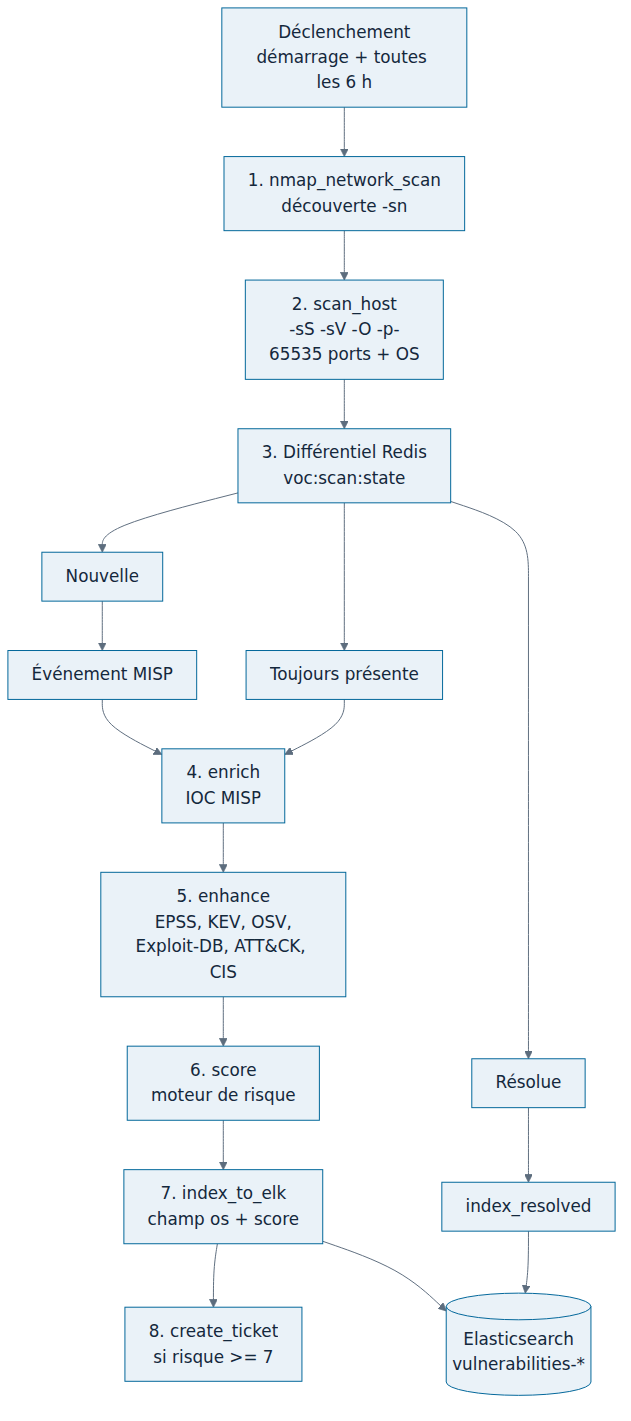
\includegraphics[width=0.68\linewidth,keepaspectratio]{diagrams/pipeline.png}
\caption{Pipeline de scan, enrichissement et indexation des vuln\'erabilit\'es}
\end{figure}

\subsection{Description des \'etapes}

\begin{center}
\small
\begin{longtable}{@{}l >{\raggedright\arraybackslash}p{0.66\linewidth}@{}}
\toprule
\textbf{\'Etape} & \textbf{Description} \\
\midrule
\endhead
\bottomrule
\endlastfoot
\texttt{nmap\_network\_scan} & T\^ache p\'eriodique (d\'emarrage + toutes les
6\,h) qui d\'ecouvre les h\^otes actifs avec \texttt{nmap -sn} et renvoie la
liste des h\^otes. \\
\texttt{scan\_host} & Scan complet par h\^ote : \texttt{nmap -sS -sV
--version-intensity 5 -O -p- -T4}, c'est-\`a-dire l'\textbf{int\'egralit\'e
des 65535 ports TCP}, la version des services et la \textbf{d\'etection du
syst\`eme d'exploitation} (\texttt{osmatch}). Le champ \texttt{os} est
transmis au document index\'e. \\
\texttt{process\_network\_results} & Rappel du \emph{chord} : compare les
r\'esultats \`a l'\'etat m\'emoris\'e (\texttt{voc:scan:state} dans Redis) et
classe chaque cl\'e \texttt{h\^ote|cve|port} en \emph{nouvelle},
\emph{toujours pr\'esente} ou \emph{r\'esolue}, puis d\'eclenche le
sous-pipeline adapt\'e. \\
\texttt{enrich} & Recherche MISP (\texttt{restSearch}) de la CVE et
rattachement des IOC correspondants. \\
\texttt{enhance} & Enrichissement approfondi : EPSS, CISA KEV, OSV,
Exploit-DB, VirusTotal, classification OWASP, tactiques/techniques MITRE
ATT\&CK, rem\'ediation, durcissement CIS et liste de v\'erifications. \\
\texttt{score} & Appel du moteur de risque (\texttt{POST /score}) pour
calculer le score 0--10 et la s\'ev\'erit\'e. \\
\texttt{index\_to\_elk} & Envoi du document enrichi (y compris le champ
\texttt{os}) \`a Logstash (\texttt{:5044}), qui l'achemine vers l'indice
\texttt{vulnerabilities-AAAA.MM.JJ}. \\
\texttt{create\_ticket} & Cr\'eation d'un ticket GLPI si
\texttt{risk\_score >= 7}, avec une checklist en suivi. La d\'edouplication
(\texttt{find\_existing\_ticket}) v\'erifie l'absence de ticket ouvert pour
le m\^eme (\texttt{h\^ote}, \texttt{CVE}). \\
\texttt{sync\_glpi\_to\_elk} & T\^ache horaire qui synchronise l'\'etat des
tickets GLPI vers l'indice \texttt{glpi-*} pour les tableaux de bord. \\
\bottomrule
\end{longtable}
\end{center}

\subsection{Analyse diff\'erentielle}

L'\'etat de chaque d\'ecouverte est repr\'esent\'e par une cl\'e
\texttt{h\^ote|cve|port} stock\'ee dans Redis. \`A chaque cycle :

\begin{itemize}[leftmargin=1.6em]
  \item une cl\'e absente de l'\'etat pr\'ec\'edent est class\'ee
        \textbf{nouvelle} (cr\'eation d'un \'ev\'enement MISP, enrichissement
        complet, ticket si le risque est suffisant) ;
  \item une cl\'e pr\'esente dans les deux \'etats est class\'ee
        \textbf{toujours pr\'esente} (r\'e-enrichissement sans doublon de
        ticket ou d'\'ev\'enement) ;
  \item une cl\'e pr\'esente pr\'ec\'edemment mais absente maintenant est
        class\'ee \textbf{r\'esolue} (\texttt{index\_resolved}).
\end{itemize}

Ce m\'ecanisme permet de mesurer l'\'evolution du risque dans le temps et
d'\'eviter la duplication des tickets.

\subsection{Synchronisation GLPI $\rightarrow$ ELK}

\begin{figure}[htbp]
\centering
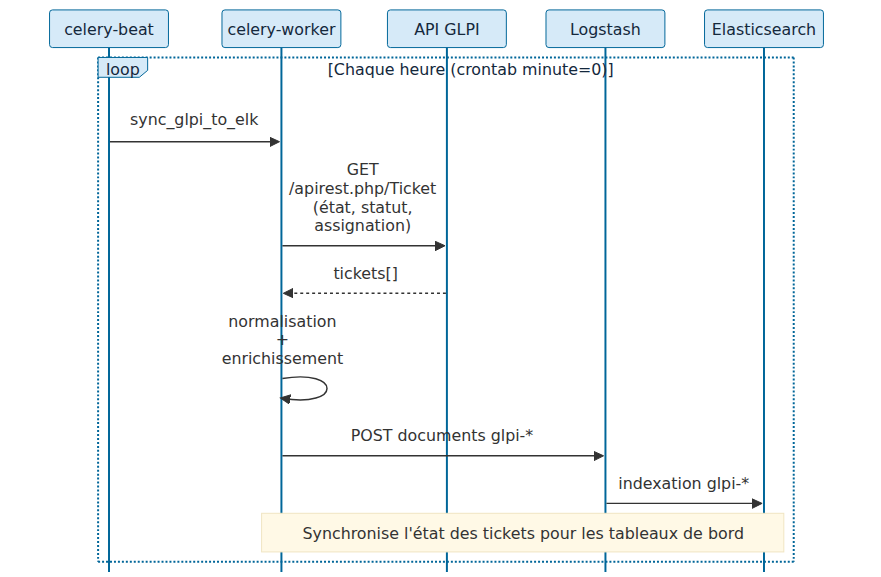
\includegraphics[width=0.85\linewidth,keepaspectratio]{diagrams/glpi_sync.png}
\caption{Synchronisation horaire de l'\'etat des tickets GLPI}
\end{figure}

\subsection{Ordonnancement et files}

\begin{center}
\small
\begin{tabularx}{\linewidth}{@{}l l X@{}}
\toprule
\textbf{T\^ache} & \textbf{Planification} & \textbf{Description} \\
\midrule
\texttt{nmap\_network\_scan} & d\'emarrage + \texttt{0 */6 * * *} & Scan complet du sous-r\'eseau + diff\'erentiel \\
\texttt{sync\_glpi\_to\_elk} & \texttt{0 * * * *} (horaire) & Synchronisation des tickets GLPI vers ELK \\
\bottomrule
\end{tabularx}
\end{center}

Les t\^aches sont rout\'ees vers des files RabbitMQ d\'edi\'ees :

\begin{center}
\small
\begin{tabularx}{\linewidth}{@{}l l X@{}}
\toprule
\textbf{T\^ache} & \textbf{File} & \textbf{R\^ole} \\
\midrule
\texttt{discovery} / \texttt{scan\_host} & \texttt{scan} & D\'ecouverte et scan (nmap) \\
\texttt{enrich} / \texttt{enhance} & \texttt{enrich} & Enrichissement intelligence \\
\texttt{score} & \texttt{score} & Calcul du score de risque \\
\texttt{index\_to\_elk} & \texttt{index} & Envoi vers Logstash/Elasticsearch \\
\texttt{create\_ticket} & \texttt{ticket} & Cr\'eation des tickets GLPI \\
\bottomrule
\end{tabularx}
\end{center}

La configuration du worker est la suivante :

\begin{lstlisting}[language=bash,caption={Commande du worker Celery}]
celery -A tasks worker --loglevel=info --concurrency=2 \
    -Q scan,enrich,score,index,ticket
\end{lstlisting}

\clearpage

% ===========================================================================
% 8. MOTEUR DE RISQUE
% ===========================================================================
\section{Moteur de calcul du risque}

Le moteur de risque est un service FastAPI sans \'etat qui transforme la note
CVSS brute en un score de risque orient\'e \emph{m\'etier} en appliquant des
bonus li\'es au contexte.

\subsection{Entr\'ees}

\begin{center}
\small
\begin{tabularx}{\linewidth}{@{}l l X@{}}
\toprule
\textbf{Champ} & \textbf{Intervalle} & \textbf{Signification} \\
\midrule
\texttt{cvss\_base} & 0--10 & Note CVSS de base \\
\texttt{is\_critical\_asset} & bool\'een & L'actif est critique pour l'activit\'e \\
\texttt{misp\_threat\_active} & bool\'een & Intelligence de menace active (MISP) \\
\texttt{exploit\_available} & bool\'een & Un exploit public existe \\
\texttt{network\_exposure} & 0--1 & Facteur d'exposition r\'eseau \\
\texttt{epss\_score} & 0--1 & Probabilit\'e d'exploitation EPSS \\
\texttt{in\_kev} & bool\'een & Pr\'esence dans le catalogue CISA KEV \\
\bottomrule
\end{tabularx}
\end{center}

\subsection{Algorithme de notation}

\begin{center}
\small
\begin{tabularx}{\linewidth}{@{}X l@{}}
\toprule
\textbf{Condition} & \textbf{Bonus} \\
\midrule
Note de base & \texttt{cvss\_base} \\
\texttt{is\_critical\_asset} & $+$ \texttt{cvss\_base} $\times 0.5$ \\
\texttt{misp\_threat\_active} & $+$ 2.0 \\
\texttt{exploit\_available} & $+$ 1.5 \\
\texttt{network\_exposure} $> 0$ & $+$ \texttt{network\_exposure} $\times 2$ \\
\texttt{in\_kev} & $+$ \texttt{RISK\_KEV\_BOOST} (2.0 par d\'efaut) \\
\texttt{epss\_score} $\geq$ seuil (0.5) & $+$ \texttt{RISK\_EPSS\_BOOST} (1.0 par d\'efaut) \\
\midrule
\textbf{Note finale} & $\min(\text{score}, 10)$ \\
\bottomrule
\end{tabularx}
\end{center}

\begin{center}
\small
\begin{tabular}{lc}
\toprule
\textbf{S\'ev\'erit\'e} & \textbf{Intervalle de score} \\
\midrule
\textcolor{vocred}{Critique} & $\geq 9$ \\
\textcolor{vocorange}{\'Elev\'ee} & $\geq 7$ et $< 9$ \\
\textcolor{blue}{Moyenne} & $\geq 4$ et $< 7$ \\
\textcolor{vocgreen}{Faible} & $< 4$ \\
\bottomrule
\end{tabular}
\end{center}

\subsection{Sch\'ema de d\'ecision}

\begin{figure}[htbp]
\centering
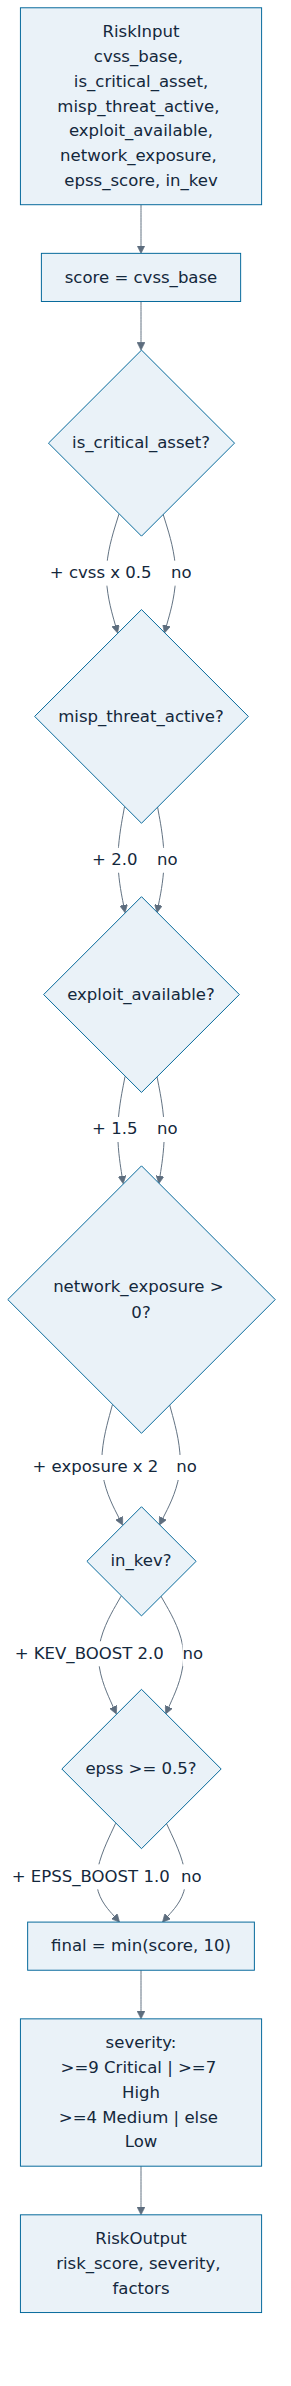
\includegraphics[width=0.6\linewidth,keepaspectratio]{diagrams/risk_engine.png}
\caption{Sch\'ema de d\'ecision du moteur de risque}
\end{figure}

\subsection{Exemples de calcul}

\textbf{Exemple 1 --} CVE-2024-6387 (OpenSSH \emph{regreSSHion}) sur un actif
critique, exploit public disponible, pr\'esente dans le catalogue KEV, score
EPSS de 0.99 et exposition totale ($= 1.0$) :

\begin{center}
\small
\begin{tabular}{l r}
\toprule
\textbf{Composant} & \textbf{Valeur} \\
\midrule
Note CVSS de base & 8.1 \\
Bonus actif critique ($8.1 \times 0.5$) & $+4.05$ \\
Bonus exploit public & $+1.5$ \\
Bonus exposition ($1.0 \times 2$) & $+2.0$ \\
Bonus KEV & $+2.0$ \\
Bonus EPSS ($0.99 \geq 0.5$) & $+1.0$ \\
\midrule
Score brut & 18.65 \\
\textbf{Score final} & \textbf{10.0} (Critique) \\
\bottomrule
\end{tabular}
\end{center}

\textbf{Exemple 2 --} Vuln\'erabilit\'e CVSS 4.3 sur un actif non critique,
sans exploit public, EPSS de 0.01, absente du KEV, exposition faible
($= 0.2$) :

\begin{center}
\small
\begin{tabular}{l r}
\toprule
\textbf{Composant} & \textbf{Valeur} \\
\midrule
Note CVSS de base & 4.3 \\
Bonus exposition ($0.2 \times 2$) & $+0.4$ \\
\midrule
Score brut & 4.7 \\
\textbf{Score final} & \textbf{4.7} (Moyenne) \\
\bottomrule
\end{tabular}
\end{center}

Ces deux exemples illustrent l'int\'er\^et du mod\`ele : une faille \`a fort
impact r\'eellement exploit\'ee est port\'ee \`a un niveau \emph{Critique},
tandis qu'une faille \`a faible exposition reste \emph{Moyenne}.

\subsection{R\`egles de cr\'eation des tickets GLPI}

\begin{itemize}[leftmargin=1.6em]
  \item Ticket cr\'e\'e uniquement si \texttt{risk\_score >= 7.0}.
  \item \textbf{Urgence} : 5 (critique) si risque $\geq 9$, sinon 4.
  \item \textbf{Impact} : 4 (toujours).
  \item \textbf{Priorit\'e} : 5 (tr\`es \'elev\'ee) si risque $\geq 7$, sinon 4.
  \item \textbf{Titre} : \texttt{[VOC] \{s\'ev\'erit\'e\} - \{CVE\} sur \{h\^ote\}}.
\end{itemize}

\clearpage
